
\paragraph{Locations of category centers.}

In the absence of language, we can infer that the shared categories we observe arise either due to innate biological factors, environmental factors such as the distribution of colors in the terrestrial environment, or a combination of the two.
The categories that we identify align well with the daylight locus (the line between the blue of the daytime sky, and the yellow of the sun, which itself closely follows the planckian locus), and also the warm/cool object/background distinction previously identified \citep{rosenthal_color_2018}. It is plausible that what we observe is the presence of two fundamental categories - `likely to be object of interest' and `likely to \emph{not} be object of interest'. 

\paragraph{Limitations of colorspace.}

For these experiments we used a nominally perceptually-uniform colorspace: CIELUV. This space has been derived psychophysically, with the goal of minimizing differences in perceptual non-uniformity across the space, for color differences of small magnitudes (the apparent color difference between two points in one part of the space should be equal to the apparent color difference between two points in another part of the space, given that the cartesian distance between the two points in each case be the same).

However, non-uniformities within the space are known to exist (ref?), and uniformity for small color differences does not necessarily assure uniformity for larger color differences (ref? Teunissen?). Likewise, uniformity for the conditions under which the psychometric measurements from which the space was determined (considering: spatial, temporal, spectral etc.) does not necessarily assure uniformity across all possible viewing conditions (ref).

With this in mind, it is reasonable to consider what the effect of residual non-uniformity might be on the results of our experiment. As discussed by \cite{panichello_error-correcting_2019} (their Figure S5) non-uniformities in colorspace could also potentially lead to systematic biases on tasks such as ours. The logic goes as follows: our points are uniformly distributed in our chosen space (\autoref{fig:StimuliAndParadigm}A), but if this space is actually non-uniform compared to the colorspace implicitly being used by an observer, then these same points will be \emph{non}-uniformly distributed in a hypothetical `perfect colorspace'. It follows that for each cue color, surrounding distractor points might actually be closer or further away than anticipated. If the nearest neighbors on one side of the cue are actually chromatically closer than the neighbors on the other side, one would expect these to be chosen at a higher frequency than the others, creating a systematic bias.

Unfortunately, these biases act in a similar fashion and are difficult to separate from one another. One potential way to distinguish one type of bias from another is to consider the theoretical relationship between bias and variance: if biases arise due to non-uniformities in colorspace, we would expect the attractor points to also have the \emph{highest} variance in responses. This is because in the hypothetical `perfect space' these points are actually tightly clustered, and so in the presence of noise we can assume that they will be frequently picked over one another. Conversely, at attractor points in spaces where the bias results from categoricality, theory would predict that we would see the \emph{lowest} levels of variance - if these points are conceptualized as `magnets' or `valleys' then we would expect cumulative noise to preferentially return to the attractor point, reducing the variance in responses.

In our data, we see...

[Compare to Bae/Panichello]

\paragraph{Saturation bias.}

Non-uniformities in CILUV may also plausibly result in our nominally iso-saturated colors actually being variably saturated. This would be a concern, as it would be a reasonable prediction that higher saturation colors would be more salient, and thus more likely to be selected as responses. In a control experiment we see no (or very little) bias towards higher saturation colors. In \autoref{fig:saturationBias} it can be seen that there are a reasonable number of errors where an animal picks a higher saturation version of the same hue (lower left quadrant), but it is also seen that the number of errors of the inverse type (upper right quadrant) are roughly equal in number.

\begin{figure}
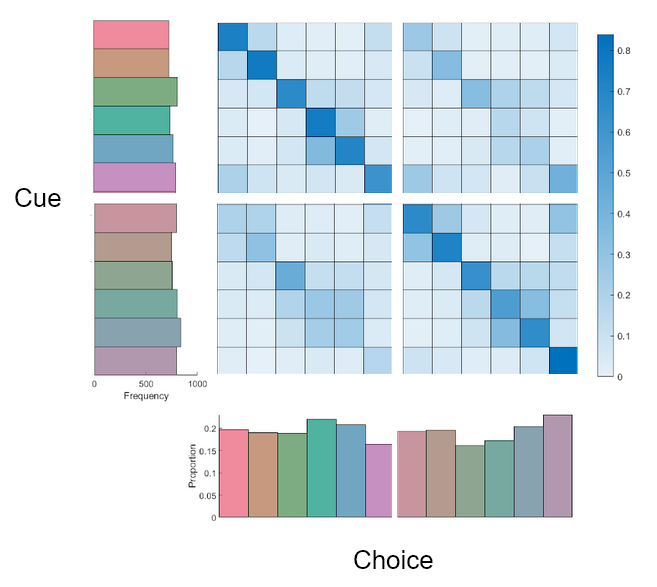
\includegraphics[width=\textwidth]{../../Figures/saturationBias.png}
\caption{\textbf{Saturation Bias.}
Heatmap of cues and corresponding choices. Selections along the negative diagonal correspond to correct choices. Choices along the negative diagonal in the bottom left and top right quadrants show trials on which an incorrect choice was made in such a way that the hue was correct but the higher or lower saturation versions of the cue were chosen (respectively). Note: the main diagonal is expected to be filled in at a greater extent regardless of performance level, since the correct choice is shown on every trial, whereas only a subset of the incorrect choices are shown.}
\label{fig:saturationBias}
\end{figure}



\paragraph{Comparison with humans} % /Panichello